\documentclass[tikz, border=6pt]{standalone}
\usepackage{tikz}
\usepackage{physics}
\usepackage{siunitx}
\usepackage{ifthen}
\usepackage{tikz}
\usepackage[outline]{contour}
\usepackage{silence}

\usetikzlibrary{calc}
\usetikzlibrary{angles,quotes}
\usetikzlibrary{arrows.meta}
\usetikzlibrary{patterns}

\AtBeginDocument{\RenewCommandCopy\qty\SI}
\tikzset{>=latex}
\contourlength{1.4pt}

% -----------------------------------------------------------------------------
% Color palette
% -----------------------------------------------------------------------------
\colorlet{angleColor}{blue!70!black}
\colorlet{forceColor}{red!65!black}
\colorlet{forceComponentColor}{red!50!blue!80!black!80}
\colorlet{sensorTrackColor}{black!50}
\colorlet{signalOutputColor}{green!70!black}
\colorlet{supplyTerminalColor}{red!70!black}
\colorlet{groundTerminalColor}{blue!70!black}
% \colorlet{uColor}{green!50!black};
% \colorlet{omegaColor}{orange!90!black};
% \colorlet{tauColor}{green!80!black};

% -----------------------------------------------------------------------------
% Reusable drawing styles (used by pendulum.tex)
% -----------------------------------------------------------------------------
\tikzset{
  supportSurface/.style={
    preaction={fill,top color=black!10,bottom color=black!5,shading angle=20},
    fill,
    pattern=north east lines,
    draw=none,
    minimum width=0.3,
    minimum height=0.6
  },
  forceVector/.style={
    ->,
    forceColor,
    very thick,
    line cap=round
  },
  information text/.style={
    rounded corners,
    fill=red!10,
    inner sep=1ex
  }
}

\usetikzlibrary{arrows.meta, patterns}

% ---------------------------------------------------------------------------
% Hybrid System Trajectory Diagram
%
% Illustrates a generic event update in a hybrid system at event time t_i:
%
%   x(t)  -- continuous state
%             Evolves smoothly between events. In the example shown here,
%             the event update resets the state from x^-(t_i) to x^+(t_i).
%
%   q(t)  -- discrete state
%             Piecewise constant; may change only at event times.
%             Open circle = pre-event value q^-(t_i)
%             Filled circle = post-event value q^+(t_i)
%
% Time grid: t_{i-1}, t_i (event), t_{i+1}
% ---------------------------------------------------------------------------

\begin{document}
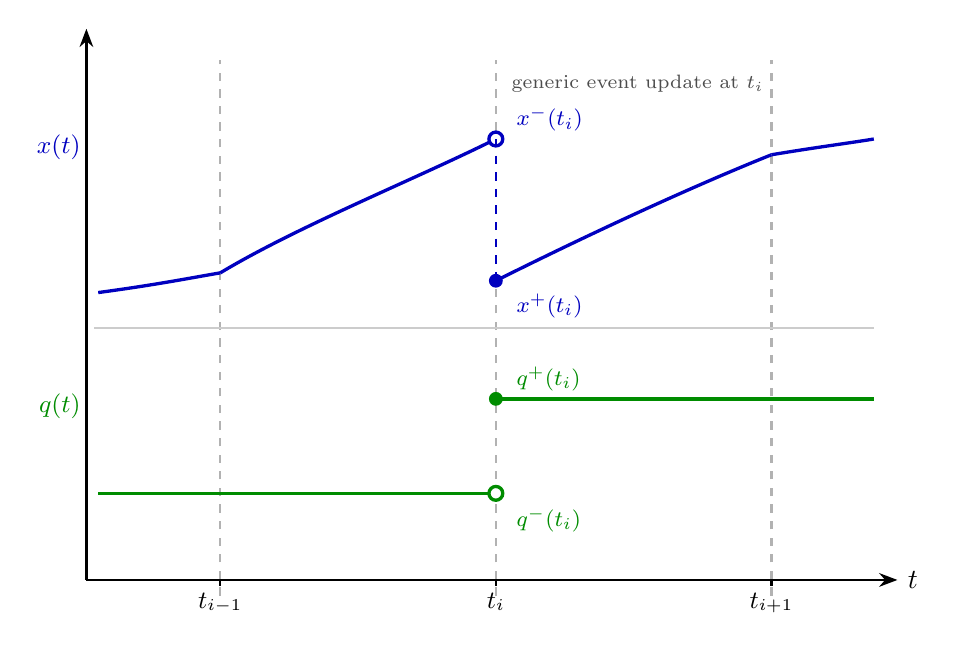
\begin{tikzpicture}[>=Stealth]

% ---------------------------------------------------------------------------
% Color aliases
% ---------------------------------------------------------------------------
\colorlet{xColor}{blue!75!black}
\colorlet{qColor}{green!55!black}

% ---------------------------------------------------------------------------
% Axes
% ---------------------------------------------------------------------------
\draw[->, thick] (0.3, 0) -- (10.6, 0) node[right] {$t$};
\draw[->, thick] (0.3, 0) -- (0.3, 7.0);

% ---------------------------------------------------------------------------
% Time-axis ticks and labels
% ---------------------------------------------------------------------------
\foreach \tx/\lbl in {2.0/{t_{i-1}}, 5.5/{t_i}, 9.0/{t_{i+1}}} {
    \draw[thick] (\tx, 0.08) -- (\tx, -0.08);
    \node[below, font=\small] at (\tx, -0.04) {$\lbl$};
}

% ---------------------------------------------------------------------------
% Dashed vertical lines at grid points
% ---------------------------------------------------------------------------
\foreach \tx in {2.0, 5.5, 9.0} {
    \draw[dashed, gray!60, thick] (\tx, -0.2) -- (\tx, 6.6);
}

\node[font=\scriptsize, text=black!70] at (7.3, 6.3) {generic event update at $t_i$};

% ===========================================================================
%  DISCRETE STATE  q(t)  -- lower band
%  Piecewise constant; may jump at event times.
% ===========================================================================
\node[left, qColor, font=\small\bfseries] at (0.35, 2.2) {$q(t)$};

% Segment before t_{i-1}
\draw[qColor, very thick] (0.45, 1.1) -- (2.0, 1.1);

% Constant segment [t_{i-1}, t_i]
\draw[qColor, very thick] (2.0, 1.1) -- (5.5, 1.1);

% Open circle at q^-(t_i)
\draw[qColor, very thick, fill=white] (5.5, 1.1) circle (2.5pt);

% Constant segment [t_i, t_{i+1}] and beyond (new level after update)
\draw[qColor, very thick] (5.5, 2.3) -- (10.3, 2.3);

% Filled circle at q^+(t_i)
\fill[qColor] (5.5, 2.3) circle (2.5pt);

% Annotations
\node[right=4pt, qColor, font=\footnotesize] at (5.5, 0.76) {$q^{-}(t_i)$};
\node[right=4pt, qColor, font=\footnotesize] at (5.5, 2.55) {$q^{+}(t_i)$};

% ===========================================================================
%  CONTINUOUS STATE  x(t)  -- upper band
%  Smooth between events; the example update at t_i causes a state jump.
% ===========================================================================
\node[left, xColor, font=\small\bfseries] at (0.35, 5.5) {$x(t)$};

% Extension before t_{i-1}
\draw[xColor, very thick]
    (0.45, 3.65)
    .. controls (1.2, 3.75) and (1.7, 3.85) ..
    (2.0, 3.9);

% Smooth segment [t_{i-1}, t_i] ending at x^-(t_i)
\draw[xColor, very thick]
    (2.0, 3.9)
    .. controls (3.0, 4.5) and (4.5, 5.1) ..
    (5.5, 5.6);

% Open circle at x^-(t_i)
\draw[xColor, very thick, fill=white] (5.5, 5.6) circle (2.5pt);

% Dashed vertical connector: visualizes the instantaneous state update
\draw[xColor, thick, dashed] (5.5, 5.6) -- (5.5, 3.8);

% Filled circle at x^+(t_i)
\fill[xColor] (5.5, 3.8) circle (2.5pt);

% Smooth segment [t_i, t_{i+1}] departing from x^+(t_i)
\draw[xColor, very thick]
    (5.5, 3.8)
    .. controls (6.7, 4.4) and (8.0, 5.0) ..
    (9.0, 5.4);

% Extension after t_{i+1}
\draw[xColor, very thick]
    (9.0, 5.4)
    .. controls (9.6, 5.5) and (10.0, 5.55) ..
    (10.3, 5.6);

% Annotations
\node[right=4pt, xColor, font=\footnotesize] at (5.5, 5.85) {$x^{-}(t_i)$};
\node[right=4pt, xColor, font=\footnotesize] at (5.5, 3.48) {$x^{+}(t_i)$};

% ---------------------------------------------------------------------------
% Thin separator between bands (visual guide only)
% ---------------------------------------------------------------------------
\draw[black!20, thin] (0.4, 3.2) -- (10.3, 3.2);

\end{tikzpicture}
\end{document}
